\documentclass[pdf, intlimits, 12pt, unicode]{beamer} %Для Latex2Pdf  tex -> pdf

%Пакеты для русского языка
\usepackage[T2A]{fontenc}
\usepackage[utf8]{inputenc}
\usepackage[english,russian]{babel}

%Пакет для вставки рисунков
\usepackage{graphicx}
%AMS TEX значки и пр.
\usepackage{amssymb}
\usepackage{amsthm}
\usepackage{amssymb, amsmath, amsthm, amsfonts, amscd, geometry}


%Привычный шрифт для математических формул
\usefonttheme[onlymath]{serif}

%Нужно включать, если используется "тема" (стиль оформления) по умолчанию
\usepackage{beamerthemesplit}

%Общий стиль ("тема") оформления слайдов
%Требование: черные буквы на белом фоне
\usetheme{Warsaw}

\addtobeamertemplate{navigation symbols}{}{%
    \usebeamerfont{footline}%
    \usebeamercolor[fg]{footline}%
    \hspace{1em}%
    \insertframenumber/\inserttotalframenumber
}
\setbeamercolor{footline}{fg=black}
\setbeamerfont{footline}{series=\bfseries}

%Более крупный шрифт для подзаголовков титульного листа
\setbeamerfont{institute}{size={\fontsize{13}{16}}}
\setbeamerfont{frametitle}{size={\fontsize{16}{19}}}

%Задание команды (\bluetext) для выделения конкретным (синим) цветом
%(используйте \alert для выделения цветом выбранной "темы")
%\setbeamercolor{bluetext_color}{fg=blue}
%\newcommand{\bluetext}[1]{{\usebeamercolor[fg]{bluetext_color}#1}}


\newcommand{\Expect}{\mathbb E}
\newcommand{\PRob}{\mathbb P}
\newcommand{\leqs}{\leqslant}
\newcommand{\geqs}{\geqslant}
\newcommand{\eps}{\varepsilon}
\DeclareMathOperator{\re}{Re}
\DeclareMathOperator{\I}{I}


\newtheorem*{theoremm}{Теорема}
\newtheorem*{lemmaa}{Лемма}
\newtheorem*{cons}{Следствие}
\newtheorem*{notee}{Замечание}



%Если используется последовательное появление пунктов списков на слайде
%(не злоупотребляйте в слайдах для защиты дипломной работы), чтобы
%еще непоявившиеся пункты были все-таки немножко видны.
%\setbeamercovered{transparent}

\title{Рост двудольных графов с~рёберным приоритетом}
\author{Ерохин Станислав Евгеньевич, гр. 512}
\institute{
	\vspace{0.30cm}\\
    Научный руководитель: к.ф.-м.н., д. Якубович~Ю.~В. \\
    Рецензент: к.ф.-м.н., д. Валландер С.\,С. \\
}
\date{
}

\begin{document}

\begin{frame}
    \titlepage
\end{frame}

\begin{frame}
    \frametitle{BitTorrent}
    Протокол для кооперативного обмена файлами через интернет -- BitTorrent:
    \begin{itemize}
        \item создан в 2001 году,
        \item сейчас более 30\% трафика.
    \end{itemize}
    \medskip
    \medskip
    
    Отличительные особенности:
    \begin{itemize}
		\item файл делится на фрагменты,
		\item клиенты обмениваются фрагментами;
		\item изначально файл только у одного клиента.
    \end{itemize} 
\end{frame}

\begin{frame}
	\frametitle{Двудольный граф и BitTorrent}
	\begin{figure}[t]
		\vspace*{-0.4in}
		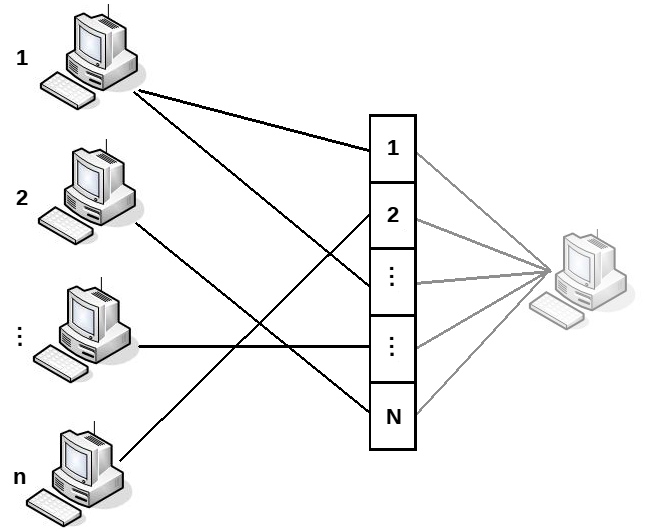
\includegraphics[scale=0.4]{clients}
		\vspace*{-0.2in}
	\end{figure}
	Доли: клиенты и фрагменты. 
	Ребра: наличие фрагмента. \\
	Модель кодирует, как выбираются фрагменты.\\
	$G_m$ --- граф на шагу $m$.
\end{frame}

\begin{frame}
	\frametitle{Двудольный граф и BitTorrent}
	Следим за минимальной степенью фрагмента: $Q(G)$.\\
	
	Почему именно за ней:
	\begin{itemize}
		\item если $Q(G)$ достаточно большая, то мала вероятность "потерять" файл;
		\item влияет на характер обмена фрагментами между клиентами.
	\end{itemize}
	Выбираем $q \in (0,1)$ и
	хотим узнать такой момент $m$, что~$Q(G_m) \geqs qn$.
\end{frame}


\begin{frame}
	\frametitle{Модели}
	Функция $Q(G_m)$ существенно зависит от алгоритма выбора очередного ребра. \\
	Хотим придумать "идеальный"\ алгоритм.
 
	\bigskip

	Было рассмотрено 3 модели:
	\begin{itemize}
		\item Равномерный выбор очередного ребра.
		\item Выбор клиента, затем выбор ребра.
		\item Выбор клиента, ребро к редкому фрагменту.
	\end{itemize}
	
	\medskip
	В каждой модели найдем такое $m$, чтобы $\PRob\big(Q(G_m) \geqs qn\big)$ была близка к единице.\\
	Считаем лучшей ту модель, в которой это число меньше.
	
\end{frame}



\begin{frame}
	\frametitle{Полученные оценки}

\begin{theoremm}[Для первой модели]
	Пусть $q, \sigma \in (0, 1)$. Возьмем 
		\vspace{-3.5mm}
		\begin{align*}
		& m = \min(nN, \lceil pnN + 2\sqrt{pnN} \rceil), \quad \text{ где} \\
		& p \geqs q + c + \sqrt{c^2+2qc}, \quad c = \frac{\ln(2N) - \ln(\sigma)}{n}.
		\end{align*}
		\vspace{-6.5mm}
		
	Тогда в графе $G_m$ с вероятностью, большей, чем $1 - \sigma$, все фрагменты будут скачены хотя бы $qn$ клиентами:
		\vspace{-3.5mm}
		\begin{equation*}
		\PRob\big(Q(G_m) \geqs qn\big) > 1 - \sigma.
		\end{equation*}
\end{theoremm}

\end{frame}

\begin{frame}
	\frametitle{Полученные оценки}
	\begin{theoremm}[Для второй модели]
		Пусть $q, \sigma \in (0, 1)$. Положим $c = \frac{\ln(2N) - \ln(\sigma)}{n}$.
		Возьмем произвольное такое число $p$, что 
			\vspace{-3mm}
			\begin{align*}
			& p \geqs q + s(p, N) + c + \sqrt{c^2+2(q+s(p, N))c}.
			\end{align*}
			\vspace{-7mm}
			
		Здесь $s(p,N) = \PRob(X \geqs N)$, где $X \in \Pi(pN)$. Положим
			\vspace{-3mm}
			\begin{align*}
			m = \min(nN, \lceil pnN + 2\sqrt{pnN} \rceil).
			\end{align*}
			\vspace{-7mm}
			
		Тогда в графе $G_m$ с вероятностью, большей, чем $1 - \sigma$, все фрагменты будут скачены хотя бы $qn$ клиентами:
			\vspace{-3mm}
			\begin{equation*}
			\PRob\big(Q(G_m) \geqs qn\big) > 1 - \sigma.
			\end{equation*}
	\end{theoremm}

	\begin{cons}
		Если $(q+c) < \frac{1}{4}$, то неравенство на $p$ заменяется на:\\
		\quad\quad\quad\quad\quad\quad\quad
		$p \geqs 2\left(q + c + \exp\left(-\frac{N}{18}\right) \right)$.
	\end{cons}
\end{frame}


\begin{frame}	
	\frametitle{Полученные оценки}
	\begin{theoremm}
		Пусть $q \in \big[0, \frac{1}{5} - \frac{2}{n}\big]$. 
		Возьмём $m \geqs (qn + 2) N$, тогда~в~графе $G_m$ с~вероятностью большей, 
		чем~$1 - n\exp\left(-\frac{N}{5}\right) +  \exp\left(- \frac{N}{20}\right)$, все фрагменты 
		скачены~как~минимум $qn$ клиентами:
		\vspace{-3mm}
		\begin{equation*}
		\PRob\Big( Q(G_m) \geqs qn \Big) > 1 - n\exp\left(-\frac{N}{5}\right) +  \exp\left(- \frac{N}{20}\right).
		\end{equation*}
	\end{theoremm}
	
	\begin{notee}
		Пусть $q \in [0,1]$. Тогда, если мы возьмём $m < qnN$, то в~любом графе $G$, в котором ровно $m$ ребер, точно будет фрагмент, 
		со степенью меньшей $qn$, т.е. $Q(G_m) < qn$.
	\end{notee}

\end{frame}

\begin{frame}
	\frametitle{Эрдеш--Реньи}
	Эрдеш и Реньи предложили случайные графы $G_{n, p}$ и $G_{n, m}$.
	\begin{itemize}
		\item $G_{n,m}$ --- в графе на $n$ вершинах проводится $m$ ребер.
		\item $G_{n,p}$ --- каждое ребро проводится с вероятностью $p$.
	\end{itemize}
	Известны леммы об асимптотической эквивалентности этих графов для монотонных свойств.
	
	\bigskip
	
	Наш граф $G_m$ в модели 1 --- двудольный аналог графа~$G_{n,m}$.
	Для доказательства оценок в первой модели нами вводился граф $H_p$ --- аналог $G_{n,p}$.
	
	Была доказана лемма об эквивалентности для монотонных свойств графов~$G_m$~и~$H_p$.
	
	
\end{frame}


\begin{frame}
	\frametitle{Лемма о монотонном свойстве}
	\begin{lemmaa}
		Пусть $A$ --- множество всех графов, которые обладают некоторым монотонным свойством, а $\delta \in (0,1)$.
		Тогда, если $\PRob( H_p \in A) \geqs 1 - \eps$, то
			\vspace{-3mm}
			\begin{equation*} \label{l1_1}
			\PRob(G_{\lceil pnN(1+\delta) \rceil} \in A) > 1 - \frac{\eps}{1 - \exp\left(-\frac{\delta^2}{4}pnN\right)},
			\end{equation*}
			\vspace{-7mm}
			
		a если $\PRob( H_p \in A) \leqs \eps$, то
			\vspace{-3mm}
			\begin{equation*}\label{l1_2}
			\PRob(G_{\lfloor pnN(1-\delta) \rfloor} \in A) < \frac{\eps}{1 - \exp\left(-\frac{\delta^2}{2}pnN\right)}.
			\end{equation*}
	\end{lemmaa}

\end{frame}
\end{document}
